\chapter{Justification and Evaluation}


\section{Justification}

The relevance of deploying advanced machine learning models for financial markets cannot be overstated, especially in the context of cryptocurrency markets with their inherent volatility, unpredictability, and the significant financial opportunities it presents. Cryptocurrencies, unlike traditional financial assets, exhibit swift price fluctuations and unique market dynamics, driven by a myriad of factors ranging from technological advancements to regulatory changes and investor sentiment. This unpredictability, while posing considerable risks, also opens up substantial opportunities for market participants equipped with the right tools to interpret and anticipate market movements.\\

In this high-stakes environment, a well-crafted predictive model can serve as a powerful tool, offering users a significant edge. By harnessing advanced machine learning techniques to analyze and interpret market data, such models can uncover hidden patterns and trends that may elude traditional analysis, enabling users to make more informed, data-driven decisions.\\

Furthermore, the successful implementation of this framework in the cryptocurrency domain lays a robust foundation for its application in other financial markets. The model's adaptability and learning capabilities could potentially be extended to traditional fiat currencies, such as the US Dollar or Euro, and even equities, thereby broadening the scope of its applicability and impact. In essence, this research not only addresses the immediate challenges posed by the cryptocurrency market but also paves the way for additional financial modeling and analysis techniques that could provide significant insights in market operations. \\

In a domain where timely and accurate information is paramount, the development of such predictive models is not merely an academic exercise but a necessary evolution to meet the complex demands of modern financial markets. This research is a step towards realizing that goal, offering promising avenues for both immediate application in the cryptocurrency market as well as potential future expansions. \\

Central to the designed framework is the comprehensive data collection system, which serves as the lifeblood for any machine learning application. By ensuring the availability of high-quality, real-time market data, the framework sets the stage for precise and insightful market predictions. \\

Key to the framework's utility is its focus on continuous improvement. The systematic training and fine-tuning of the model's hyperparameters are instrumental in adapting to the market's evolving dynamics. This iterative approach not only refines the models accuracy over time but also embeds a culture of perpetual enhancement within the framework's architecture. The incorporation of robust experiment tracking mechanisms ensures that each iteration is documented, paving the way for transparent and informed advancements in the model's development. \\

The practical implications of this framework extend far beyond its technical footprint. For traders and investors, the framework promises a new platform for data-driven insights. This is achieved by harnessing the predictive power of advanced machine learning techniques. The framework offers a tool that can potentially uncover market trends and investment opportunities that might be obscure or latent in raw market data. This level of analysis can empower traders and investors with a more nuanced understanding of market movements, enabling them to make more informed and strategic decisions. \\

Moreover, the framework's modular and adaptable architecture ensures that it can remain at the forefront of technological advancements. As new machine learning techniques and analytical tools emerge, the framework is well-positioned to integrate these innovations, continually enhancing its predictive capabilities. \\

In essence, this research is not just about building a sophisticated predictive model, it is about crafting a dynamic, evolving tool that grows in intelligence and insight. It is about offering traders and investors a lens through which the complexities of the cryptocurrency market are not just seen, but also understood and anticipated. The real-world benefits, therefore, are not only imminent but also potentially transformative, redefining the landscape of financial decision-making in the digital age. \\

\subsection{Future Scope}

As the framework continues to evolve, the integration and enhancement of its core components present promising avenues for advancement. A significant leap forward would involve the consolidation of the Rust backend and the model service, morphing them into a singular, powerful entity within the system. This transformation is not merely about streamlining the architecture but also about harnessing the full potential of Rust's performance, stability, and memory safety features. \\

The Rust ecosystem is rapidly gaining momentum in the domain of machine learning. Libraries such as Burn \cite{burnDev}, PyO3 \cite{PyO3PythonFromRust}, and TensorFlow bindings \cite{tensorflowRust} for Rust are laying the groundwork for a new paradigm in machine learning infrastructure, one where Rust's efficiency and robustness can be leveraged to its full extend. The strategic integration of these libraries and technologies could redefine the framework's operational efficiency, making it a formidable tool in processing and analyzing large volumes of financial data. \\

The envisioned future of this framework is one where Python's versatility in machine learning is combined with Rust's performance-oriented nature. This synergy aims to reduce the framework's dependency on Python, not by displacing it, but by optimizing the computational-intensive aspects of the system with Rust's capabilities. Such an approach promises not only a boost in performance but also an enhancement in the system's reliability and resource efficiency.

Furthermore, this evolution is not just about technological transformation but also about positioning the framework at the forefront of innovation in financial analytics. As machine learning continues to advance, the framework's adaptable and forward-looking architecture ensures it remains relevant and capable of incorporating cutting-edge methodologies and tools. 
\\
In conclusion, the road map for the framework's development is clear and ambitious. It involves not just incremental improvements but a strategic reorientation towards a more integrated, efficient, and cutting-edge system. This vision, when realized, will not only enhance the framework's capabilities but also redefine its role and impact in the domain of financial market analytics.
 
\section{Evaluation}

\subsection{Methodology Assessment}
Detailed in Section \ref{section:model_evaluation} it becomes evident that the current models, despite their sophisticated architecture, fall short of the accuracy and reliability required to guide users in making sound financial decisions. The performance limitations are underscored by the metrics used: Mean Absolute Error (MAE), Mean Squared Error (MSE), Explained Variance Score, R-squared Score, Root Mean Squared Error (RMSE), and Mean Absolute Percentage Error (MAPE). While these metrics provide a quantitative measure of the model's predictive capabilities, their collective insights suggest that the models may not fully capture the complexities of the cryptocurrency market dynamics. \\ 

The reliance on these metrics, primarily centered around error minimization and variance explanation, might be insufficient to holistically evaluate the model's predictive performance. In the context of financial decision-making, where the cost of false positives and false negatives can be high, it is crucial to consider metrics that reflect the model's ability to balance precision and recall. Incorporating Precision, Recall, and the F1-score into the evaluation framework could provide a more nuanced understanding of the model's performance, particularly in terms of their ability to accurately predict significant market movements. \\

Precision would offer insight into the model's ability to minimize false positives, a critical factor when predicting price movements in volatile markets. Recall would shed light on the model's ability to accurately identify actual positive occurrences, which is essential to ensure no significant investment opportunities are missed. Lastly, the F1-score, as a harmonic mean of precision and recall, would provide a single metric to assess the balance between precision and recall, offering a more balanced view of the model's predictive accuracy. \\

In addition to the conventional evaluation metrics utilized, it is crucial to consider the dynamic nature of model performance during training. Monitoring the evolution of model loss throughout the training process, alongside visualizing the performance on the validation set, can provide valuable insights into the model's learning trajectory.  \\
The absence of a specified seed for \texttt{TensorFlow} and \texttt{numpy} during the model tuning process introduces an element of unpredictability, hindering the re-producibility of model training. To enhance the robustness of model tuning the establishment of a seed would ensure consistency across different runs. By incorporating these practices, the evaluation framework would gain significant depth, offering a more comprehensive understanding of the model's predictive capabilities, and aiding in the refinement of future model iterations.

\subsection{Data Quality and Reliability}
The data collection mechanism, established through the Kraken Websocket API, has demonstrated reliability and consistency during the testing phase, underscoring the robustness of the underlying infrastructure. However, there are opportunities to fortify the system further and enhance the data's integrity and utility. \\

One notable limitation is the system's current inability to manage unexpected interruptions such as connection timeouts or errors. The absence of an automated re-connection protocol could lead to gaps in the data, potentially undermining the model's training and predictive accuracy. Implementing a monitoring mechanism for heartbeat signals from the API and logging any anomalies could significantly mitigate this risk. By documenting instances of potential data loss and promptly re-establishing connections, the system would be able to ensure a more continuous and reliable data stream. \\

Additionally, the data aggregation strategy should be refined to maximize flexibility and granularity. While the current framework aggregates data on an hourly basis, providing the capability to create Open, High, Low, Close (OHLC) aggregates on a 1-minute basis and subsequently aggregating these into larger time frames (e.g., 5 minutes, 15 minutes, 1 hour, etc.) on demand would offer enhanced granularity. This flexibility would not only cater to diverse analytical needs but also enable more nuanced model training. \\

Moreover, integrating core metrics such as moving averages directly into the database aggregation process, rather than computing them in the model service, could streamline operations and provide direct access to these key indicators. This integration would not only reduce computational overhead in the model service, but also offer potential for real-time analytical insights, enhancing the user experience by providing immediate access to these critical metrics. \\

In conclusion, while the data collection and processing mechanisms exhibit a strong foundation, the proposed enhancements in error handling, data aggregation flexibility, and integration of core metrics into the database would elevate the system's robustness and precision. These improvements are pivotal in ensuring that the data infrastructure can support more advanced predictive models and ultimately lead to a more informed and effective decision-making processes. \\

\subsection{Infrastructure}
The technology stack, despite its robust architecture and comprehensive suite of services, encounters a notable bottleneck with Timescale's performance. This issue persists despite the implementation of indexes aimed at optimizing query efficiency, indicating a more complex challenge. \\

The system's infrastructure is extensive: a Node.js/Angular frontend hosted in a Docker container with Nginx using multiple workers, an MLflow webserver and model service both operating with multiple workers, a multi-threaded Rust backend with one thread dedicated to continuous data collection, and MinIO providing S3 storage services. This multifaceted setup places considerable demand on the CPU, particularly in the context of a development environment concurrently running applications like VS Code and Chrome. \\

In light of these insights, the observed latency in Timescale might be attributed to the cumulative load from the various services and the development environment itself, rather than the database's intrinsic limitations. Transitioning to a dedicated server for Timescale, equipped with robust hardware specifications, is anticipated to alleviate this bottleneck significantly. This would ensure that the database's performance is optimized, without being hindered by the extensive computational demands of the diverse services and development tools. \\

Moreover, the model tuning script, crucial for refining the predictive models, currently operates locally due to complexities in integrating a Jupyter notebook server with CUDA in a docker container. This setup, while necessary for harnessing GPU acceleration, does not align with the mentality of this research to utilize Docker for enabling the framework to run anywhere.\\

By addressing these infrastructure challenges and optimizing the computational allocation, the system could achieve a harmonious balance between its extensive components, ensuring seamless performance and robust support for cryptocurrency market analysis and predictions. \\

\subsection{Model}

To evaluate the LSTM models performance properly, two baseline models, Moving Average (MA) and Last Value, were established. This comparative analysis was aimed at providing a comprehensive understanding of the LSTM's capabilities in the context of predictive analytics. The Last Value model (Figure \ref{fig:last_value_forecast}), serving as a rudimentary baseline, operates under a simple premise predicting future values based solely on the most recent observation. Surprisingly, this approach demonstrated significant efficacy, reflected in its superior performance metrics: it achieved the lowest Mean Squared Error (MSE) at 23.52, the lowest Mean Absolute Error (MAE) at 3.24, and the highest R\(^2\) Score and Explained Variance Score, both at 0.975 (Table \ref{tab:metrics_comparison}). Such outcomes not only highlight the Last Value models effectiveness but also challenge the conventional wisdom that more complex models inherently offer better forecasting accuracy. This is particularly noteworthy in scenarios where the latest data point is a strong predictor of future trends. \\

\begin{figure}[H]
    \centering
    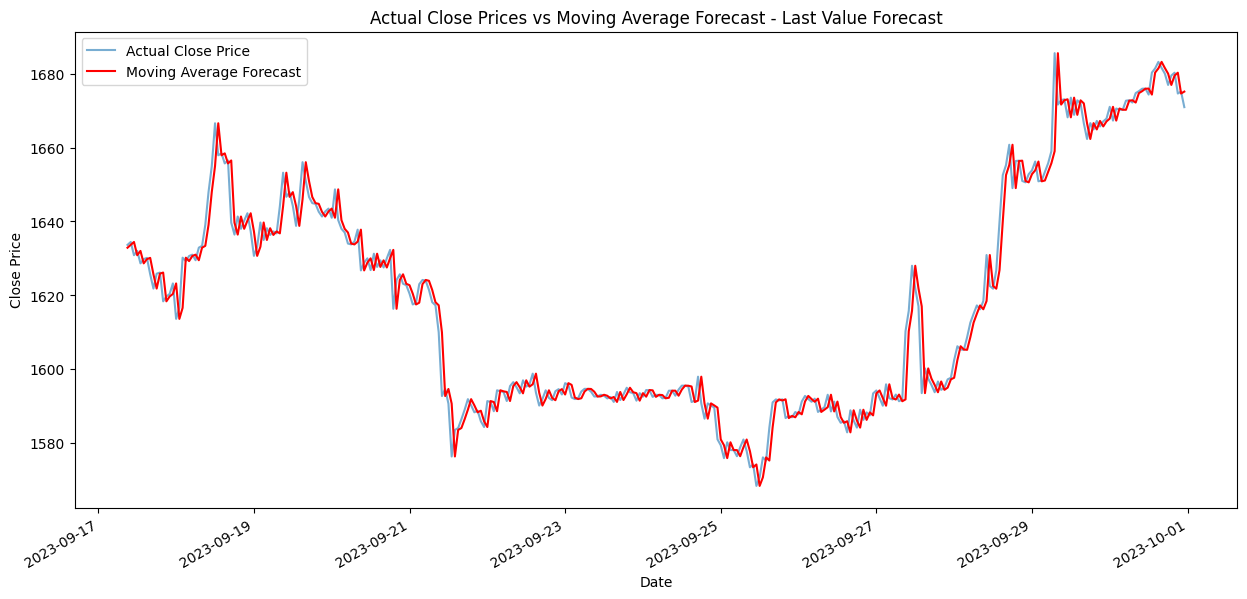
\includegraphics[width=\textwidth]{figures/last_value_model_forecast.png}
    \caption{Last Value Forecast Performance}
    \label{fig:last_value_forecast}
\end{figure}


The Moving Average model (Figure \ref{fig:ma_model_forecast}), which calculates predictions based on the average of the last five data points, was selected as a slightly more sophisticated baseline. Despite its simplicity, it too yielded impressive results (Table \ref{tab:metrics_comparison}), with an MSE of 46.54 and an MAE of 4.41. Its R\(^2\) Score and Explained Variance Score, both at 0.951, further attest to its capability to adequately capture the underlying trends in the data. These findings underscore the potential of simple statistical methods to provide reliable forecasts, challenging the premise that advanced models are always necessary for accurate predictions. \\

\begin{figure}[H]
    \centering
    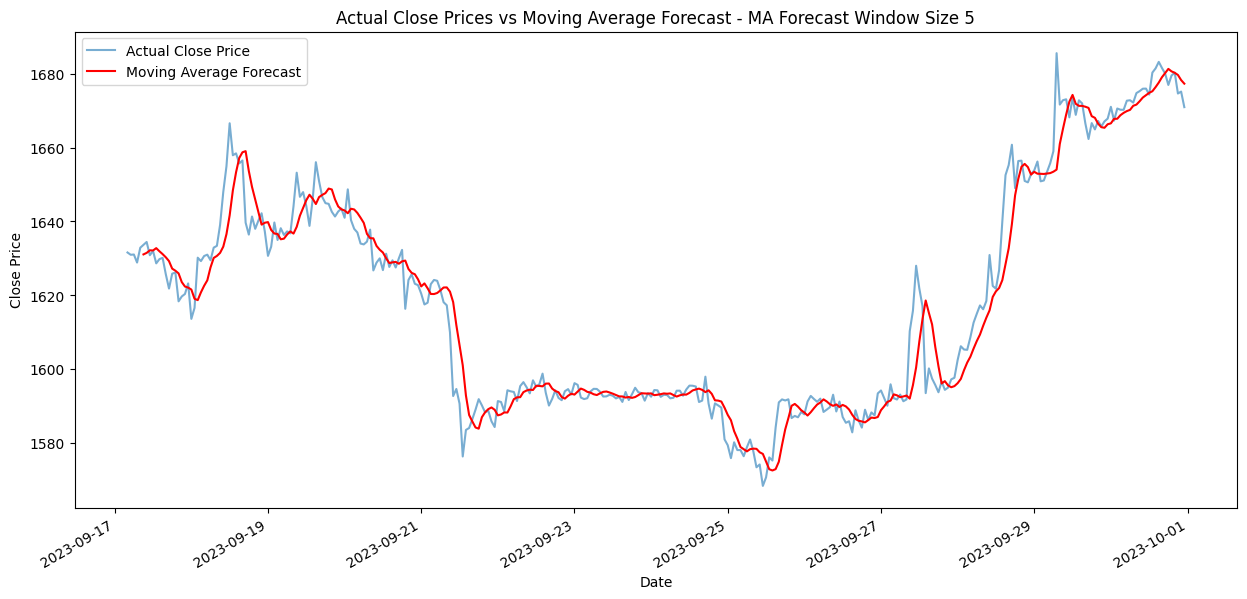
\includegraphics[width=\textwidth]{figures/ma_model_forecast.png}
    \caption{Moving Average Model Forecast Performance}
    \label{fig:ma_model_forecast}
\end{figure}

In contrast, the LSTM model, designed to leverage long-term dependencies in data, exhibited lower performance relative to the baseline models (Table \ref{tab:metrics_comparison}). With the highest MSE of 121.07, an MAE of 8.74, and the lowest R\(^2\) Score of 0.88, the LSTM's results were somewhat disappointing. This underperformance raises important considerations regarding the application of complex neural networks like LSTMs in forecasting tasks, especially when simpler models can achieve comparable or superior results under certain conditions. \\ 


\begin{table}[H]
\centering
\begin{tabular}{|l|c|c|c|}
\hline
Metric & Moving Average & Last Value & LSTM (clean-mare-368) \\ 
\hline
Mean Squared Error & 46.54 & 23.52 & 121.07 \\
Mean Absolute Error & 4.41 & 3.24 & 8.74 \\
Root Mean Squared Error & 6.82 & 4.85 & 11 \\
Mean Absolute Percentage Error& 27.18\% & 19.94\% & 54.04\% \\
R\(^2\) Score & 0.951 & 0.975 & 0.88 \\
Explained Variance Score & 0.951 & 0.975 & 0.897 \\
Timesteps & 327 & 327 & 327 \\
\hline
\end{tabular}
\caption{Comparison of Metrics Across Three Models}
\label{tab:metrics_comparison}
\end{table}

The consistent timesteps across all models ensure a level playing field for comparison, further validating the conclusions drawn from the data. This research illustrates the vital lesson that in forecasting, simpler models can not only serve as valuable benchmarks but can also outperform more complex algorithms under certain conditions. It emphasizes the need for careful consideration of model selection, based on the characteristics of the dataset and the specific forecasting objectives, rather than defaulting to more sophisticated models. The findings advocate for a nuanced approach to predictive modeling, where the choice of model is informed by empirical performance metrics and the theoretical understanding of the dataset's dynamics.